\chapter{GPU Implementierung}

\section{Einleitung}

Nachdem das theoretische und numerische Fundament gelegt wurde, soll nun auf die GPU-Implementierung eingegangen werden.
Dieser Abschnitt bezieht sich auf den grundlegenden Algorithmus, welcher im Rahmen der Master-Arbeit basierend auf einer bestehenden
CUDA-Implementierung von [] übernommen, erweitert und optimiert wurde.
Die zusätzlich eingeführten  Immersed Boundary Methoden werden ausführlich in Abschnitt () behandelt.

\section{GPU Architektur}
- karten varianten c1060 und tesla k20m , datasheet im anhang

-In Abbildung () ist exemplarisch das Speicherlayout der cuda karte dargstellt .
-Hierbei sei angemerkt das dies in keiner weise dem hardware layou entspricht aber als model
-für verständnis der algoritmhus am besten
-z.b. ist der local memory auf der karte im global memory speicherbereich

- lese paper / präsi zur optimierung
- geschwindigkeiten
- shared vs global etc

\begin{figure}[!bp]
  \centering
  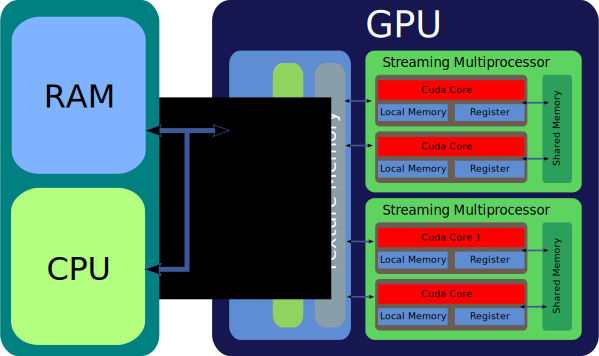
\includegraphics[width=0.8\textwidth]{gfx/cuda/gpu.png}\label{fig:gpu_arch}
  \caption{Speicherlayout einer Nvidia-GPU}
\end{figure}

-bild
-speicher bereiche
-grid layout function call
-threadidx etc

\section{Algorithmus}
-oder so ?
-erläuterung  implementierung
-speicherverwaltung

\section{Optimierung}
- coalesceded
- bank conflicts?
- teilvolumen nicht rechnen

\section{Validierung}
- beispiel rayleigh benard system
- masa
- vgl o2 vs o4 masa cube
- bifurcation


\newpage

